There is a chip on each dot in Fig. 1.6. In one move, you may simultaneously move any two chips by one place in opposite directions. The goal is to get all chips into one dot. When can this goal be reached?
\begin{center}
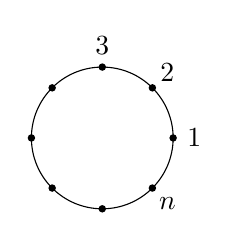
\begin{tikzpicture}[scale=0.9]
\draw (0,0) circle (1);
\foreach \a in {0,45,...,315} \fill (\a:1) circle (1.5pt);
\node at (0:1.3) {$1$}; \node at (45:1.3) {$2$}; \node at (90:1.3) {$3$}; \node at (-45:1.3) {$n$};
\end{tikzpicture}

Fig. 1.6
\end{center}
